\section{Overview}
The team has been set with a task to design and make a project based on the PYNQ board that would process a camera input in real time and use that as an input into an interactive application. The group has decided that creating a game, with the purpose of entertaining the user would be the best idea. 

The team started exploring different approaches to this task. One of the initial ideas was to make a game similar to Draw with friends, where it flashes a word and the person has to draw the word, while the other person is guessing. After some consideration, the group has decided against that idea because it would require very careful hand motion tracking, which would be complex.

	In the end, the decision has been made to go with a game, which the team called “CookEIE monster”. The idea of the game is to catch cookies with your mouth and avoid broccoli. The player will have 3 lives and if he comes into contact with broccoli, life would be lost. When the life counter reaches 0, the game is over. A player can restart the game at anytime by covering the camera completely.


The goals for this project would be:
\begin{itemize}
  \item Produce a python game interface
  \item Use object recognition techniques to detect a mask (which would be worn by the player on their face, so that the system could detect it).
  \item If the previous step is successful, extend the capabilities to detecting a face and if the mouth is open or not.
  \item The output FPS to be no lower than 24.
\end{itemize}

\section{High level overview}


Each frame, the camera output is being stored into an image buffer on the PYNQ board’s RAM. The FPGA will access and analyse this data, outputting two integer coordinates and one boolean value. The procedure in the FPGA can be divided into two main parts: Processing and Detection. 

All the algorithms in this section were implemented in Javascript as a proof of concept (see Appendix A.6 for code).

First, using multi-level thresholding\cite{resma2018multilevel}, the group wants to separate pixels that fall in a predefined colour range by making them white (Hex FFFFFF) while making all other pixels black (Hex 000000) (see figure \ref{edge detection}).



\begin{figure}[h]
\centering
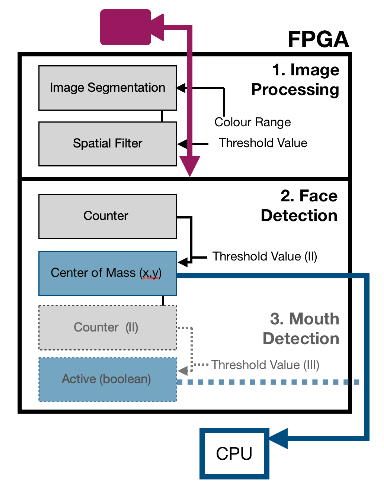
\includegraphics[scale=1]{schematic}
\caption{Block diagram of the project.}
\label{schematic}
\end{figure}

\begin{figure}[H]
    \centering
    \begin{subfigure}[b]{0.45\textwidth}
        \centering
        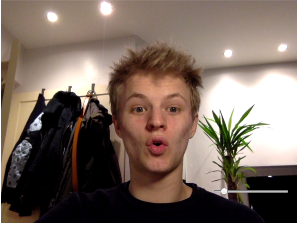
\includegraphics[width=\textwidth]{chrispre}
        \caption{Pre processing.}
        \label{chrispre}
    \end{subfigure}
    \hfill
    \begin{subfigure}[b]{0.45\textwidth}
        \centering
        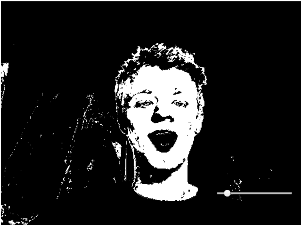
\includegraphics[width=\textwidth]{chrispost}
        \caption{Post processing.}
        \label{chrispost}
    \end{subfigure}
    \hfill
    \caption{Face detection algorithm.}
    \label{edge detection}
\end{figure}


To get the right colour range, the group sampled multiple skin tones under different light conditions, producing the following range: (see Figure \ref{colorrange})

\begin{figure}[H]
\centering
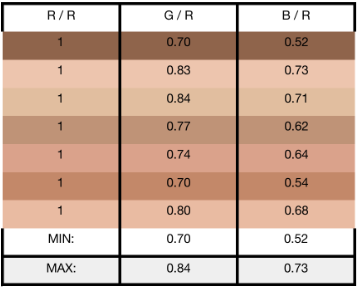
\includegraphics[scale=1]{colorrange}
\caption{Ratio of green and blue RGB values to red for different skin tones.}
\label{colorrange}
\end{figure}

The table shows the ratios of the green and blue values compared to the red value of each sample. By looking at the ratio range of RGB values instead of the range of each RGB colour, the group hopes to minimize problems concerning the light condition and thus achieve more accurate thresholding.

Next, a spatial filter\cite{nguyen2012} will be applied in order to minimize the number of white pixels in the background. This can be done by locating the neighbours of each white pixel, presumably in sizes of 3x3\cite[p.12]{nelson}, and changing all pixels in that group to black if the amount of white pixel is below a threshold of 50\%. As with all predefined values in this description, this threshold value will likely be adapted during testing.

Since groups of one pixel now have the same colour, the image resolution could possibly be decreased by a factor of 9 so that would result in a better performance. Furthermore, both thresholding and the spatial filter could be combined by only making a pixel white if 50\% of its neighbours are in the defined colour range (see Figure \ref{threshold}).


\begin{figure}[H]
    \centering
    \begin{subfigure}[b]{0.45\textwidth}
        \centering
        
\includegraphics[width=\textwidth]{img1}
        \caption{Below threshold.}
        \label{below}
    \end{subfigure}
    \hfill
    \begin{subfigure}[b]{0.45\textwidth}
        \centering
        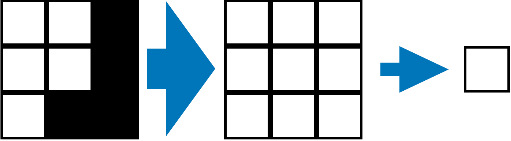
\includegraphics[width=\textwidth]{img2}
        \caption{Above threshold.}
        \label{above}
    \end{subfigure}
    \hfill
    \caption{Spatial filter example.}
    \label{threshold}
\end{figure}

In the second stage, a counter counts all the white pixels and decides if a face is present or not by comparing it to a predefined threshold\cite[p.23]{inproceedings}. If that threshold is surpassed, the centre of mass of all white pixels is calculated, detecting the face of the player and returning its x and y value. 

\begin{figure}[H]
\centering
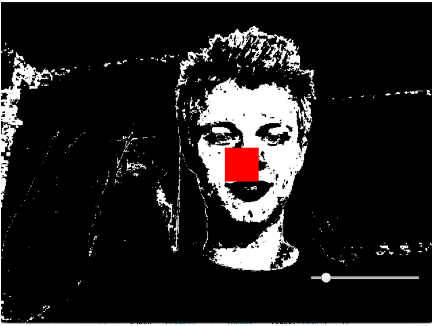
\includegraphics[scale=1]{final1}
\caption{Calculated center of mass represented with red square.}
\label{schematic}
\end{figure}

The final step the group considers is detecting the mouth of the player. This could be done by finding the height of the black cluster underneath the centre of the face. If that height is bigger than a predefined threshold, the function returns true, else wise it returns false.

\section{Expected Outcome}

The team by the end of the project aims to have achieved a system which recognises the player's mouth to play the game. For this to happen first the code for face detection has to be made, and from there the team can move onto recognizing the mouth of the player. With that, all completed to a high standard, where the frame rate is high and the recognition works all the time, the signal can then be processed by the CPU. In this, the python code should be able to create a game of falling cookies after the camera has been turned completely black, which would indicate a restart for the game. Here when the cookies fall the signal from the image processing unit should be used as input. When the cookies touch the hitboxes of the mouths, they will be “eaten”. The player will need to avoid falling broccoli, otherwise would lose a life. When all the 3 lives have been lost the game is over.  All of this should happen in real time to keep in line with the specification. To end the game, the black card should be brought in front of the camera again. 

	Initially, the team will only use a ‘Cookie Monster’ mask. This should be easily recognisable due to the blue colouring. If this works well, a step can be taken to move this down to the mouth. At first, this will just a be a hitbox, so no matter if the mouth is open or closed, the hitbox will still be there. Therefore, the overall aim of the project is to make the hitbox on the mouth and to make it disappear if the mouth is closed. If this is successful, this could be extended to 2 players. In the top corner of the game will be the player's score, 1 point per cookie. In the top left will be the lives the player is one. Each player starts with 3 lives. 

	Another aspect of the game the team wants to achieve is having the sprites fall at different speeds. This will add a level of difficulty to the game. As the game goes on the faster on average each item will fall. Below is a crude diagram of the final UI design of the game (see Figure \ref{UI}). 


\begin{figure}[h]
\centering
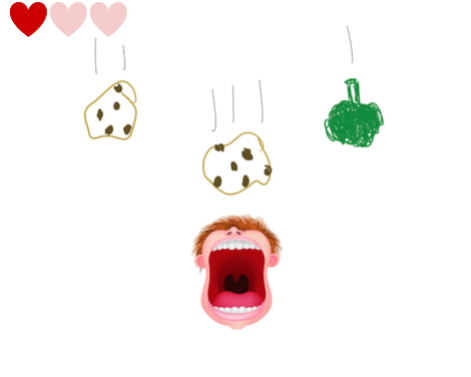
\includegraphics[scale=1]{UI}
\caption{Sketch of the UI of the game.}
\label{UI}
\end{figure}

\section{Project Planning}

With 60 days left on the project, The team have filled their time wisely with the Gantt chart pictured below (see Figure \ref{gantt}). When planning out the project they have distributed the focus throughout the group, playing to individual strengths in the area. One can see this more clearly by observing the key next to the Gantt chart (see Figure \ref{ganttkey}) showing; Edward Harriss will be focused on python (making the game), Christoph Renschler will be focused on the C code (detection of objects than later on the face), and Nikita Belenkov will be focused on hardware usage (optimising the project to hit the minimum 24FPS performance).

	In the week leading up to the holidays, each member of the team will research their respected area. This is so the team can start the coding as soon as possible over the holidays. In the long run, this will stop the backlog of work during term time and allow the team to optimise the code better once all of the members are together. The team believes this is the best solution to make better use of our time. It also allows plenty of time to troubleshoot any major and minor errors that the team will come across.

	Once the team has regathered from the holidays, they will meet up and start optimisation and testing. This will last a week. The reason behind this decision is simple: on presentation day, the team wants to put forward their best work which works fully with very limited bugs. Also from experience of the group, on big projects like this, a lot of bugs need to be ironed out before the submission.

	One may have observed from the Gantt chart the final project spans 55 days throughout the holiday. This is so while the team is working upon the project they can collect ideas and take notes. Once the project is completed a week before the deadline, the team can arrange their ideas and notes into a report and presentation. Overall the team believes this is the best strategy to perform with the complexity of this project. 


\begin{figure}[H]
    \centering
    \begin{subfigure}[b]{0.25\textwidth}
        \centering
        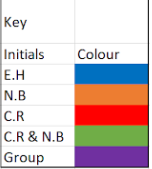
\includegraphics[width=\textwidth]{key}
        \caption{Colour key.}
        \label{key}
    \end{subfigure}
    \hfill
    \begin{subfigure}[b]{0.7\textwidth}
        \centering
        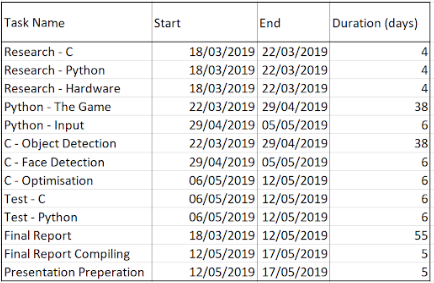
\includegraphics[width=\textwidth]{key1}
        \caption{Gantt Breakdown}
        \label{key1}
    \end{subfigure}
    \hfill
    \caption{Gantt chart explanation.}
    \label{ganttkey}
\end{figure}

\begin{figure}[h]
\centering
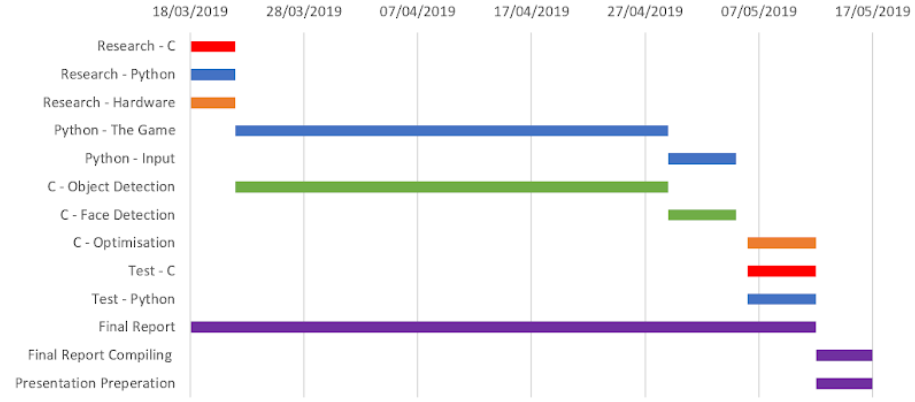
\includegraphics[scale=0.6]{gantt}
\caption{Planned gantt chart}
\label{gantt}
\end{figure}




